%%%%%%%%%%%%%%%%%%%%%%%%%%%%%%%%%%%%%%%%%%%%%%%%%%%%%%%%%%%%%%%%%%%%%%%%%%%%%%%%
%  Document class
%%%%%%%%%%%%%%%%%%%%%%%%%%%%%%%%%%%%%%%%%%%%%%%%%%%%%%%%%%%%%%%%%%%%%%%%%%%%%%%%
\documentclass[final]{siamltex}

%%%%%%%%%%%%%%%%%%%%%%%%%%%%%%%%%%%%%%%%%%%%%%%%%%%%%%%%%%%%%%%%%%%%%%%%%%%%%%%%
%  Packages and styles
%%%%%%%%%%%%%%%%%%%%%%%%%%%%%%%%%%%%%%%%%%%%%%%%%%%%%%%%%%%%%%%%%%%%%%%%%%%%%%%%
\usepackage{graphicx}
\usepackage{cite}
\usepackage{color} 
\usepackage{algorithmic}
\usepackage{algorithm}
\usepackage{epsfig}
\usepackage{xspace}
\usepackage{amsfonts}
\usepackage{amsmath}
\usepackage{amssymb}
\usepackage{url}
\usepackage{listings}
\bibliographystyle{siam}

%%%%%%%%%%%%%%%%%%%%%%%%%%%%%%%%%%%%%%%%%%%%%%%%%%%%%%%%%%%%%%%%%%%%%%%%%%%%%%%%
%  PLoS stuff
%%%%%%%%%%%%%%%%%%%%%%%%%%%%%%%%%%%%%%%%%%%%%%%%%%%%%%%%%%%%%%%%%%%%%%%%%%%%%%%%
\topmargin 0.0cm
\oddsidemargin 0.5cm
\evensidemargin 0.5cm
\textwidth 16cm 
\textheight 21cm
\usepackage[labelfont=bf,labelsep=period,justification=raggedright]{caption}
\makeatletter
\renewcommand{\@biblabel}[1]{\quad#1.}
\makeatother
\date{}
\pagestyle{myheadings}


%%%%%%%%%%%%%%%%%%%%%%%%%%%%%%%%%%%%%%%%%%%%%%%%%%%%%%%%%%%%%%%%%%%%%%%%%%%%%%%%
%  Some useful commands
%%%%%%%%%%%%%%%%%%%%%%%%%%%%%%%%%%%%%%%%%%%%%%%%%%%%%%%%%%%%%%%%%%%%%%%%%%%%%%%%
\newcommand{\oh}[1]
    {\mbox{$ {\mathcal O}( #1 ) $}}
\newcommand{\eqn}[1]
    {(\ref{eqn:#1})}
\newcommand{\fig}[1]
    {Figure~\ref{fig:#1}}
\newcommand{\tabl}[1]
    {Table~\ref{tab:#1}}
\newcommand{\tab}[1]
    {Table~\ref{tab:#1}}
\newcommand{\figs}[1]
    {Figures~\ref{fig:#1}}
\newcommand{\cuda}
    {{\sc cuda}\xspace}
\newcommand{\namd}
    {{\sc namd}\xspace}
\newcommand{\acemd}
    {{\sc acemd}\xspace}
\newcommand{\fenzi}
    {{\sc fenzi}\xspace}
\newcommand{\mdcore}
    {{\tt mdcore}\xspace}


%%%%%%%%%%%%%%%%%%%%%%%%%%%%%%%%%%%%%%%%%%%%%%%%%%%%%%%%%%%%%%%%%%%%%%%%%%%%%%%%
%  Title, author and affiliations
%%%%%%%%%%%%%%%%%%%%%%%%%%%%%%%%%%%%%%%%%%%%%%%%%%%%%%%%%%%%%%%%%%%%%%%%%%%%%%%%
\title{Efficient and Scalable Algorithms for Smoothed Particle Hydrodynamics on Multi-Core
    Architectures}
\author{Pedro Gonnet\thanks{School of Engineering and Computing Sciences,
    Durham University, Durham, Untied Kingdom ({\tt pedro.gonnet@durham.ac.uk}).}}

\begin{document}

%%%%%%%%%%%%%%%%%%%%%%%%%%%%%%%%%%%%%%%%%%%%%%%%%%%%%%%%%%%%%%%%%%%%%%%%%%%%%%%%
%  Set options for the listings package
%%%%%%%%%%%%%%%%%%%%%%%%%%%%%%%%%%%%%%%%%%%%%%%%%%%%%%%%%%%%%%%%%%%%%%%%%%%%%%%%
\lstset{%
    language=C,
    basicstyle=\small\tt,
    numbers=left,
    numberstyle=\tiny
    }


%%%%%%%%%%%%%%%%%%%%%%%%%%%%%%%%%%%%%%%%%%%%%%%%%%%%%%%%%%%%%%%%%%%%%%%%%%%%%%%%
%  Title and Author
%%%%%%%%%%%%%%%%%%%%%%%%%%%%%%%%%%%%%%%%%%%%%%%%%%%%%%%%%%%%%%%%%%%%%%%%%%%%%%%%
% Title must be 150 characters or less
\maketitle


%%%%%%%%%%%%%%%%%%%%%%%%%%%%%%%%%%%%%%%%%%%%%%%%%%%%%%%%%%%%%%%%%%%%%%%%%%%%%%%%
%  Abstract
%%%%%%%%%%%%%%%%%%%%%%%%%%%%%%%%%%%%%%%%%%%%%%%%%%%%%%%%%%%%%%%%%%%%%%%%%%%%%%%%
\begin{abstract}
A new framework for the parallelization of Smoothed Particle Hydrodynamics (SPH)
simulations on shared-memory parallel architectures is described.
This framework relies on fast and cache-efficient cell-based neighbour-finding
algorithms, as well as task-based parallelism to achieve good scaling and
parallel efficiency on mult-core computers.
\end{abstract}


%%%%%%%%%%%%%%%%%%%%%%%%%%%%%%%%%%%%%%%%%%%%%%%%%%%%%%%%%%%%%%%%%%%%%%%%%%%%%%%%
%  Metadata
%%%%%%%%%%%%%%%%%%%%%%%%%%%%%%%%%%%%%%%%%%%%%%%%%%%%%%%%%%%%%%%%%%%%%%%%%%%%%%%%
\begin{keywords} 
smoothed particle hydrodynamics,
simulation,
task-based parallelism,
multi-cores
\end{keywords}

\begin{AMS}
15A15, 15A09, 15A23
\end{AMS}

\pagestyle{myheadings}
\thispagestyle{plain}
\markboth{P. GONNET}{EFFICIENT AND SCALABLE ALGORITHMS FOR SPH}


%%%%%%%%%%%%%%%%%%%%%%%%%%%%%%%%%%%%%%%%%%%%%%%%%%%%%%%%%%%%%%%%%%%%%%%%%%%%%%%%
%  Introduction
%%%%%%%%%%%%%%%%%%%%%%%%%%%%%%%%%%%%%%%%%%%%%%%%%%%%%%%%%%%%%%%%%%%%%%%%%%%%%%%%
\section{Introduction}

Since the past few years, due to the physical limitations
on the speed of individual processor cores, instead of
getting {\em faster}, computers are getting {\em more parallel}.
This increase in parallelism comes mainly in the form of
{\em multi-core} computers, e.g. single computers which
contain more than one computational core sharing the 
same system and memory bus.
Current commercially available systems contain up to 64
general-purpose cores, yet the number of cores per
machine is predicted to continue growing exponentially,
e.g.~following Moore's law.

In order to address increasingly larger
or more complex problems, high-performance computing software
must be able to exploit this increasing parallelism.
Parallelism and parallel codes are themselves nothing new.
Many large-scale computations, e.g.~the cosmological
simulation software {\sc gadget}, can run concurrently
on several thousands of cores.

For the past two decades, the predominant paradigm for parallel
computing has been the Message Passing Interface (MPI),
in which several cores or nodes execute the same code
in parallel, intermittently exchanging data.
Using this paradigm, large simulations are generally
parallelized using a spatial decomposition, i.e.~by assigning
each node a portion of the data.
The amount of {\em computation} local to the node is then proportional
to the amount of data it contains, e.g.~its volume, while
the amount of {\em communication} is proportional to the
amount of computation spanning two or more nodes, e.g.~its
surface.

For very large computations over a moderate number of nodes,
the cost of communication is negligible compared to the
cost of computation, thus providing good parallel efficiency.
Unfortunately, if the number of nodes increases, or 
smaller problems are considered, the surface to volume ratio
grows, and the time spent on communication will start to
dominate the entire simulation, and scaling and parallel
efficiency will break down.
Another problem is that current multi-core computers
differ in an important aspect from single-core distributed-memory
systems: Since all cores on a computer share the same memory
bus and, in most cases, parts of the cache hierarchy,
the effective memory bandwidth per core is increasingly
limited, making aspects such as memory and cache efficiency
increasingly important.

This means that small simulations, for which the
maximum degree of parallelism has been reached, will never
become any faster (case in point figure).
This also means that large systems, if they do not continue
to get larger, will also break down eventually as Moore's law
is applied to the number of cores in the system.
In order to speed up small simulations, or to continue
scaling for large simulations, new approaches to how
computations are parallelized need to be considered.

One such approach consists of considering how to better exploit the
increasingly more common type of parallelism, namely shared-memory
multi-core systems.
Although such systems can be, and are commonly, used as
``clusters in a box'' by treating each core as a separate
computer, they can also be used to achieve much finer
degrees of parallelism.

In the following, I will describe a reformulation of the
underlying algorithms for Smoothed Particle Hydrodynamics (SPH)
simulations which uses asynchronous
task-based shared-memory parallelism to achieve better parallel
performance on multi-core architectures.


%%%%%%%%%%%%%%%%%%%%%%%%%%%%%%%%%%%%%%%%%%%%%%%%%%%%%%%%%%%%%%%%%%%%%%%%%%%%%%%%
%  Algorithms, i.e. decomposition, interactions, and parallelization
%%%%%%%%%%%%%%%%%%%%%%%%%%%%%%%%%%%%%%%%%%%%%%%%%%%%%%%%%%%%%%%%%%%%%%%%%%%%%%%%
\section{Algorithms}

\begin{itemize}

    \item Most, if not all, variable-radius SPH codes use variants of
        octrees to decompose the simulation space and compute the
        interactions by traversing the list of particles and searching
        for their neighbours in the tree.
        
    \item We will proceed differently, using a hierarchical cell
        decomposition, and computing the interactions by cell pairs.
        
\end{itemize}


\subsection{Smoothed Particle Hydrodynamics}

\begin{itemize}

    \item Basic formulation with interacting particles, each with
        its own smoothing length $h_i$.
    
    \item Any particle $p_j$ is {\em within range} of a particle $p_i$
        if the distance between $p_i$ and $p_j$ is smaller or equal
        to the smoothing distance $h_i$ of $p_i$.
        Note that since particle smoothing lengths may vary, this
        association is not symmetric, i.e. $p_j$ may be in range of
        $p_i$, but not $p_i$ in range of $p_j$.
        
    \item Two distinct steps: (a) loop over all particles in range
        and compute density, and (b) loop over all particles in
        range and update physical quantities.

\end{itemize}


\subsection{Spatial decomposition}

If $h_\mathsf{max} := \max_i  h_i $ is the maximum smoothing
length of any particle in the simulation, we start by splitting
the simulation domain into rectangular cells of edge length
larger or equal to $h_\mathsf{max}$.

Given such an initial decomposition, we then generate
a list of cell self-interactions, which contains all
non-empty cells in the grid.
This list of interactions is then extended by the cell
pair interactions, i.e. a list of all non-empty cells
sharing either a face, edge, or corner.
For periodic domains, cell pair interactions need also be
specified for cell neighbouring each other across
periodic boundaries.

In this first coarse decomposition, if a particle $p_j$
is within range of a particle $p_i$, they will either be
in the same cell or in neighbouring cells, for which a
cell self-interaction or cell pair interaction has been
specified respectively.

In the best of cases, i.e.~if each cell contains
only particles with smoothing length equal to the cell
edge length, if we inspect each particle in the same
and neighbouring cells, only roughly 16\% of them
will actually be within their smoothing length of each
other \cite{ref:Gonnet2007}.
If the cells contain particles who's smoothing length
is less than the cell edge length, this ratio only
gets worse.
It therefore makes sense to refine the cell decomposition,
and we will do so recursively, bisecting each cell along
all spatial dimension if: (a) The cell contains more than
some minimal number of particles, and (b) the smoothing
length of all particles within the cell is less than half
the cell edge length.
A cell will be referred to as {\em split} if it
has been divided into sub-cells.

After the cells have been split, the cell self-interactions
of each cell can be split up into the self-interaction
of its sub-cells and the pair interactions between
them (see \fig{SplitCell}).
Likewise, the cell pair interactions between two cells
that have been split can be themselves split up into
the pair interactions of the sub-cells spanning the
original pair boundary (see \fig{SplitPair}).
If only one cell within a cell pair interaction has been
split, then the cell pair interaction is preserved, i.e. the
interactions between the particles in both cells are computed,
yet the split cell is considered as a whole.

If the cells, pair interactions, and self-interactions are split
in such a way, if two particles are within range of each other,
they will (a) either share a cell for which a cell self-interaction
is defined, or (b) they will be located in two cells which share
a cell pair interaction.
In order to identify all the particles within range of each other,
it is therefore sufficient to traverse the list of cell pair
interactions and cell self-interactions, and to compute the
interactions therein.


\begin{figure}[ht]
    \centerline{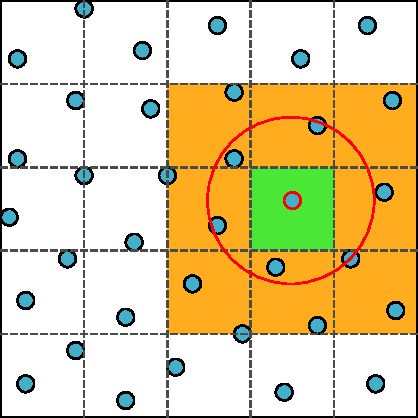
\epsfig{file=figures/InitialDecomp.pdf,height=0.3\textwidth}}
    
    \caption{Initial spatial decomposition: The space is divided into cells of
        edge length greater or equal to the largest smoothing length in the
        system. All neighbours of any given particle (small red circle) within
        that particle's smoothing length (large red circle) are guaranteed to lie
        either within that particle's own cell (green) or the directly
        adjacent cells (orange).}
    \label{fig:InitialDecomp}
\end{figure}


\begin{figure}[ht]
    \centerline{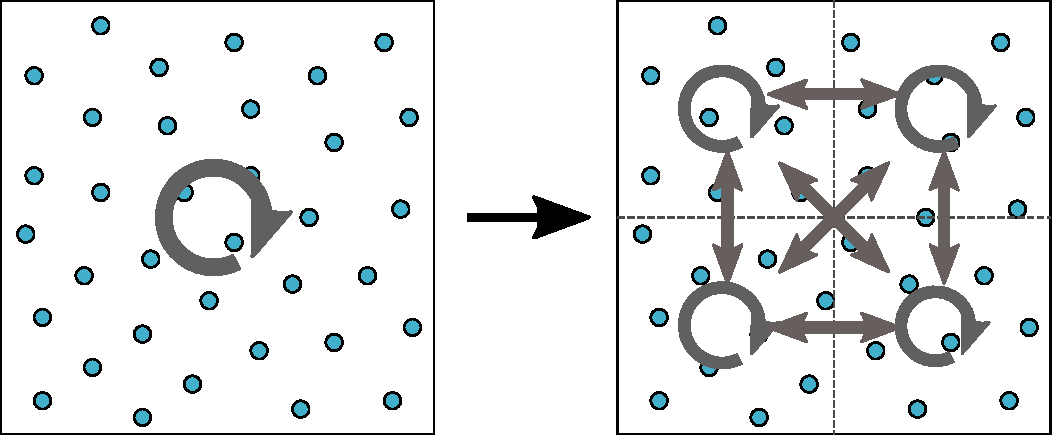
\epsfig{file=figures/SplitCell.pdf,height=0.2\textwidth}}
    
    \caption{If all particles in a cell have a smoothing length less or equal
        to half of the cell edge length, the cell can be split, and its
        self-interaction replaced by the self-interactions of its sub-cells
        and their pair interactions.}
    \label{fig:SplitCell}
\end{figure}


\begin{figure}[ht]
    \centerline{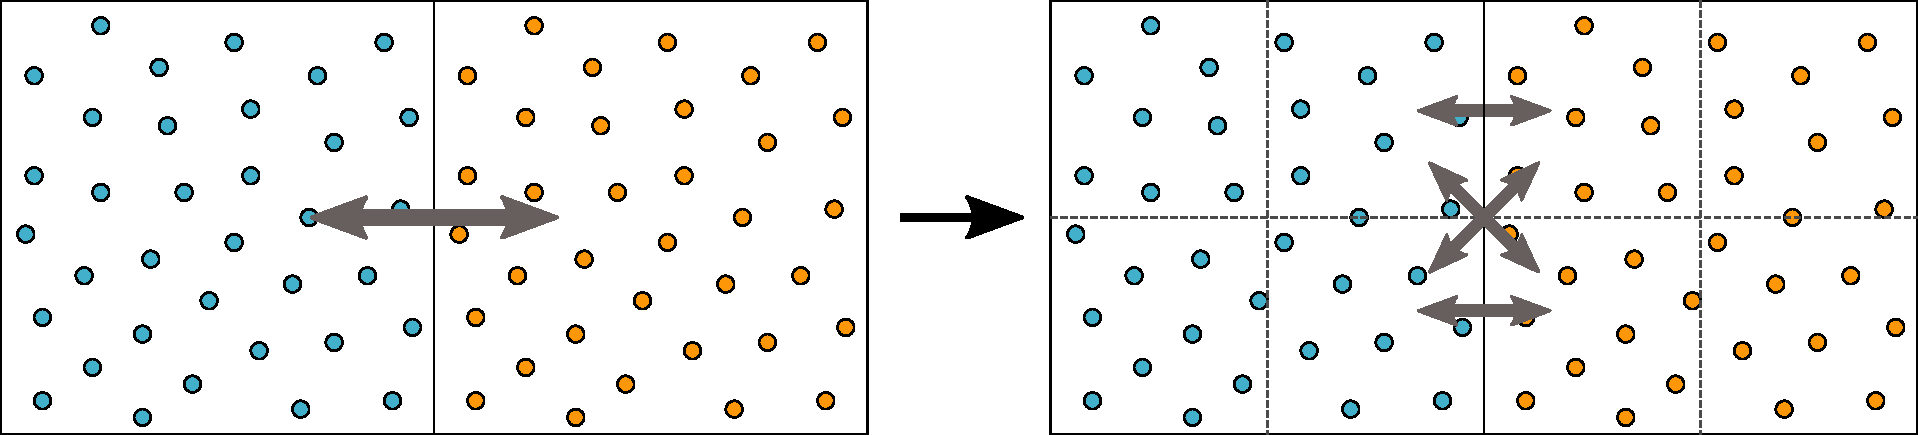
\epsfig{file=figures/SplitPair.pdf,height=0.2\textwidth}}
    
    \caption{If all particles in a pair of interacting cells have a smoothing
        length less or equal to half of the cell edge length, both cells can be
        split, and their pair interaction replaced by the pair interactions
        of the neighbouring sub-cells across the interface.}
    \label{fig:SplitPair}
\end{figure}


\subsection{Particle interactions}

The interactions between all particles within the same cell,
i.e. the cell's self-interaction, can be computed by means of
a double {\tt for}-loop over the cell's particle array.
The algorithm, in C-like pseudo code, can be written as follows:

\begin{center}\begin{minipage}{0.8\textwidth}
    \begin{lstlisting}
for ( i = 0 ; i < count-1 ; i++ ) {
    for ( j = i+1 ; j < count ; j++ ) {
        rij = ||parts[i] - parts[j]||.
        if ( rij < h[i] || rij < h[j] ) {
            compute interaction.
            update data on parts[j].
            }
        }
    update data on parts[i];
    }
    \end{lstlisting}
\end{minipage}\end{center}

\noindent where {\tt count} is the number of particles in the
cell and {\tt parts} and {\tt h} refers to an array of those
particles and their smoothing lengths respectively.
{\tt cutoff} is the cutoff distance $r_c$ used throughout the
simulation.
The particle update in line~9 stores the interaction on the
{\tt i}th particle accumulated locally in the innermost loop,
thus reducing access to the particle data.

The interactions between all particles in a pair of cells
can be computed similarly, e.g.:
   
\begin{center}\begin{minipage}{0.8\textwidth}
    \begin{lstlisting}
for ( i = 0 ; i < count_i ; i++ ) {
    for ( j = 0 ; j < count_j ; j++ ) {
        rij = ||parts_i[i] - parts_j[j]||.
        if ( rij < h_i[i] || rij < h_j[j] ) {
            compute interaction.
            update data on parts_j[j].
            }
        }
    update data on parts_i[i];
    }
    \end{lstlisting}
\end{minipage}\end{center}

\noindent where {\tt count\_i} and {\tt count\_j} refer to
the number of particles in each cell and {\tt parts\_i} and
{\tt parts\_j}, and {\tt h\_i} and {\tt h\_j}, refer to the
particles of each cell and their smoothing lengths respectively.

As described in \cite{ref:Gonnet2007}, though, using this
naive double {\tt for}-loop, only roughly $16\%$ of all particle
pairs inspected will be within range of each other, leading
to an excessive number of spurious pairwise distance evaluations.
We will therefore use the sorted cell
interactions, described therein, yet with some minor modifications, as
the original algorithm is designed for systems in which the
smoothing lengths of all particles are equal:
We first the particles in both cells along the vector joining
the centers of the two cells and then loop over the
parts $p_i$ on the left and interact them with the sorted parts $p_j$
on the right which are within $h_i$ {\em along the cell pair axis}.
The same procedure is repeated for each particle $p_j$ on the
right, interacting with each other particle $p_i$ on the
left, which is within $h_j$, {\em but not within} $h_i$, along
the cell pair axis.
The resulting algorithm, in C-like pseudo-code, looks as follows:
        
\begin{center}\begin{minipage}{0.8\textwidth}
    \begin{lstlisting}
r_i = parts_i projected onto the cell pair axis
r_j = parts_j projected onto the cell pair axis
ind_i = indices of parts_i sorted w.r.t. r_i in descending order
ind_j = indices of parts_j sorted w.r.t. r_j in ascending order
for ( i = 0 ; i < count_i ; i++ ) {
    for ( jj = 0 ; jj < count_j ; jj++ ) {
        j = ind_j[jj];
        if ( r_j[j] > r_i[i] + h_i[i] )
            break;
        rij = ||parts_i[i] - parts_j[j]||.
        if ( rij < h_i[i] ) {
            compute interaction.
            update data on parts_j[j].
            }
        }
    update data on parts_i[i];
    }
for ( j = 0 ; j < count_j ; j++ ) {
    for ( ii = 0 ; ii < count_i ; ii++ ) {
        i = ind_i[i];
        if ( r_i[i] < r_j[j] + h_j[j] )
            break;
        rij = ||parts_i[i] - parts_j[j]||.
        if ( rij < h_j[j] && rij > h_i[i] ) {
            compute interaction.
            update data on parts_i[i].
            }
        }
    update data on parts_j[j];
    }
    \end{lstlisting}
\end{minipage}\end{center}
        
\noindent where {\tt r\_i} and {\tt r\_j} contains the position
the particles of both cells along the cell axis, and
{\tt ind\_i} and {\tt ind\_j} contain the particle indices
sorted with respect to these positions respectively.

The particles need to be traversed twice: once to identify
all particles in range of the particles on the left, and
once to identify all particles in range of the particles on the
right, but that were not identified in the first loop,
thus the condition in line~24.
Instead of sorting the particles every time we compute the
pairwise interactions between to cells, we can pre-compute
the sorted indices along the 26 possible axes and store them
for each cell.
These sorted indices are, however, symmetric: e.g. the indices
computed for a cell interacting with a cell to its left along the
$x$-axis are the inverse of the indices required for interacting 
with the cell on its right.
We therefore only need to sort 13 sets of indices, and flip
the cells in a cell pair interaction around when the order
required is the opposite of the order stored.

This may all seem like quite a bit of sorting, especially
for the larger, higher-level cells in the simulation.
If, however, a cell is split and its sub-cells have been sorted,
the sorted indices of the higher-level cells can be constructed
by shifting and merging the indices of its eight sub-cells.
This reduces the \oh{n\log{n}} sorting to \oh{n} for merging. 


\begin{figure}[ht]
    \centerline{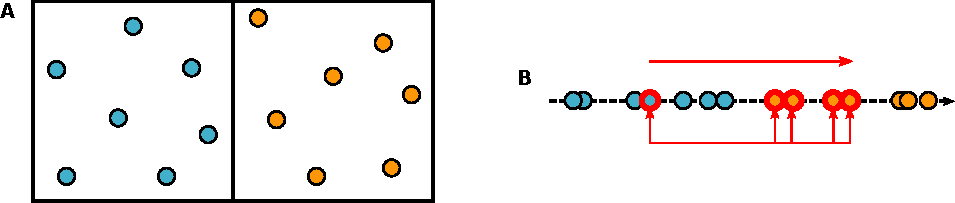
\epsfig{file=figures/SortedInteractions.pdf,width=0.7\textwidth}}
    
    \caption{Sorted cell pair interactions. ({\sf A}) Starting from a pair of
        neighbouring cells, ({\sf B}) the particles from both cells
        are projected onto the axis joining the centers of the two cells.
        The particles on the left (blue) and right (orange) are
        then sorted in descending and ascending order respectively.
        Each particle on the left is then only interacted with
        the particles on the right within the cutoff radius along the cell axis.
        }
    \label{fig:SortedInteractions}
\end{figure}


\subsection{Parallel implementation}

The arguably most well-known paradigm for shared-memory,
or thread-based parallelism, is OpenMP, in which
compiler annotations are used to describe if and when
specific loops or portions of the code can be execuded
in parallel.
When such a parallel section, e.g.~a parallel loop, is
encountered, the sections of the loop are split statically
or dynamically over the available cores.
Once all the threads have terminated, the program continues
executing in a single thread.
Unfortunately, this can lead to a lot of inefficient
branch-and-bound
type operations, which generally lead to low performance and
bad scaling on even moderate numbers of cores.

In order to better exploit shared-memory parallelism, 
we have to change the underlying paradigm, i.e. instead
of annotating an essentially serial computation with parallel
bits, describe the whole computation in a way that
is inherently parallelisable.
One such approach is {\em task-based parallelism}, in which the
computation is divided into a number of inter-dependent
computational tasks, which are then scheduled, concurrently
and aysnchronously, to a number of processors.
In order to ensure that the tasks are executed in the right
order, e.g.~that data needed by one task is only used once it
has been produced by another task, and that no two tasks
update the same data at the same time, dependencies between
tasks are specified and strictly enforced by the task
scheduler.

Several implementations of middlewares providing such task-based
parallelism exist, e.g.~Cilk, {\sc quark},
StarPU, SMP~Superscalar, OpenMP~3.0, Intel's TBB.
We will, however, differ from these approaches in that we introduce the
concept of {\em conflicts} between tasks, i.e.~not just dependencies.
Conflicts occur when two tasks operate on the same data, 
but the order in which these operations must occur is not defined.
In these previous approaches, conflicts are modeled as dependencies,
but this introduces an artificial ordering between the tasks
and imposes unnecessary constraints on the task scheduler
(see Yakota~2012 for an example of where this seriously
affects parallel performance).
These conflicts are modelled using exclusive {\em locks} on shared
resources, i.e.~a task operating on potentially shared data will
only be scheduled if can obtain an exclusive lock on that data,
thus preventing other tasks using that data to be scheduled concurrently.

The cell sorting, self interaction and pair interactions form
the three basic task types in the simulation (show a figure
showing how they are correlated).
Since the tasks are restricted to operating on the data of a
single cell, or pair of cells, two tasks conflict if they
operate on overlapping sets of cells.
The main advantage of this task decomposition is that, if
the particles are sorted according to their cellular locations,
each task only involves accessing and modifying a contained
and contiguous regions of memory, thus greatly improving their
cache efficiency (see \cite{ref:Gonnet2012} for details).
Due to the hierarchical nature of the spatial decomposition,
two tasks also conflict if they the cells of one are sub-cells
of the other.

Since the interactions have two phases, i.e.~density and force
computation, we introduce a task in between for each cell.
This ``ghost'' task depends on all the density computations
for a given cell, and, in turn, all force computations involving
that cell depend on its ghost task.
Using this mechanism, we can enforce that all density computations
for a set of particles have completed before we use this
density in the force computaitons.

The dependencies and conflicts between tasks are then given as follows:

\begin{itemize}

    \item A cell sorting task on a cell with sub-cells depends
        on the sorting tasks of all its sub-cells.

    \item A cell pair interaction depends on the cell sorting
        tasks of both its cells.
        
    \item Cell pair interaction and cell self-interaction tasks
        operating on overlapping sets of cells or sub-cells
        conflict with each other.
        
    \item The ghost task of each cell depends on all the density cell pair
        interactions and self-interactions which involve the particles
        in that cell.
        
    \item The force cell pair interaction and self-interaction tasks
        depend on the ghost tasks of the cells on which they operate.

\end{itemize}

\noindent These task dependencies are illustrated in \fig{Hierarchy} and
\fig{DensityForce}.

\begin{figure}[ht]
    \centerline{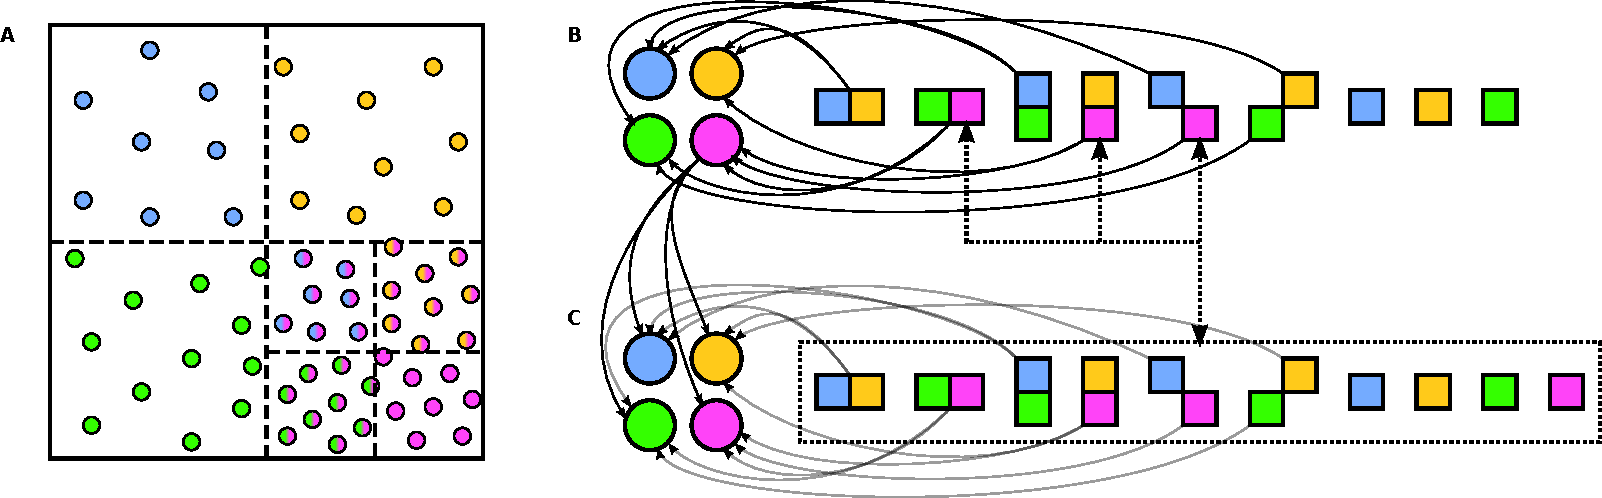
\epsfig{file=figures/Hierarchy.pdf,width=0.9\textwidth}}
    
    \caption{Task inter-dependencies: ({\sf A}) Starting from a hierarchical
        cell decomposition, ({\sf B}) the cell pair interactions (pairs
        of squares) at the highest hierarchical level depend on the sorting
        tasks (circles) of their respective cells.
        The cell self-interactions (single squares) do not depend on any
        other task. Cell pair and self-interaction tasks at the
        same level conflict when they share a common cell. The
        cell sorting tasks of each cell have no conflicts, yet
        depend on the sorting task of the next-lowest hierarchical level,
        if present.
        ({\sf C)} At the next level of hierarchy, the cell pair and
        self-interactions all conflict with the cell pair and self-interactions
        of the hierarchically superior levels (dotted arrows).
        }
    \label{fig:Hierarchy}
\end{figure}


\begin{figure}[ht]
    \centerline{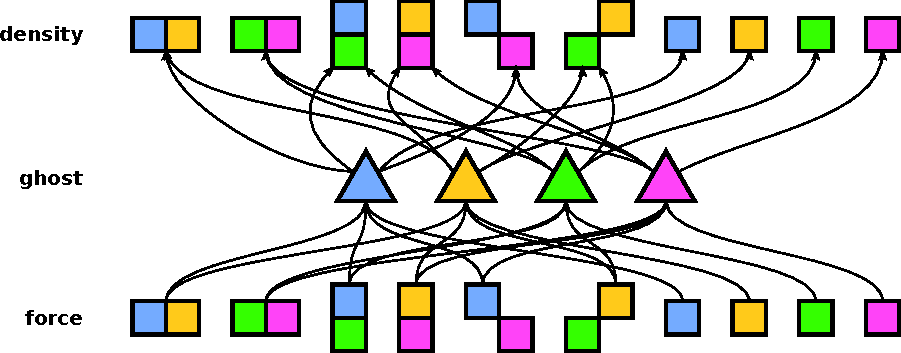
\epsfig{file=figures/DensityForce.pdf,width=0.6\textwidth}}
    
    \caption{Density and force computation: Not included in \fig{Hierarchy}
        are the two layers of cell interactions, namely once to compute
        the particle density (top row), and to compute the interaction
        forces based on the particle densities (bottom row).
        The tasks are linked by dependencies to and from ghost tasks
        (center row).
        Each ghost cell additionally depends on the hierarchically superior
        ghost tasks (not shown).
        }
    \label{fig:DensityForce}
\end{figure}


\subsubsection{Task queues}

If the dependencies and conflicts are defined correctly, then
there is no risk of concurrency problems and thus each task
can be implemented without special attention to the latter,
e.g.~it can update data without using exclusinve access barriers
or atomic memory updates.
This, however, requires some care in how the individual tasks
are allocated to the computing threads, i.e.~each task should
be allocated once to a single thread, and should not have
and unresolved dependencies, or conflict with any concurrently
executing tasks.
In the following, tasks will be stored in one or more {\em queues}:
        
\begin{center}\begin{minipage}{0.8\textwidth}
    \begin{lstlisting}
struct queue {
    int *tasks;
    int next, count;
    pthread_mutex_t lock;
    };
    \end{lstlisting}
\end{minipage}\end{center}

\noindent where {\tt tasks} is the list of task IDs in the queue, {\tt next}
is the index of the first task in the queue that has not yet been executed,
and {\tt count} is the total number of tasks, completed and waiting,
in the queue.
The {\tt pthread\_mutex\_t lock} is used to guarantee exclusive access
to the queue.

Task IDs are retreived from the queue as follows:        

\begin{center}\begin{minipage}{0.8\textwidth}
    \begin{lstlisting}
int queue_gettask ( struct queue *q , int steal ) {
    int tid, res = -1;
    pthread_mutex_lock( &q->lock );
    for ( tid = q->next ; tid < q->count ; tid++ )
        if ( q->tasks[tid] has no unresolved dependencies &&
             q->tasks[tid] can lock all the resources it needs )
            break;
    if ( tid < q->count ) {
        res = q->tasks[tid];
        if ( steal ) {
            q->count -= 1;
            swap q->tasks[tid] and q->tasks[q->count];
            }
        else {
            swap q->tasks[tid] and q->tasks[q->next];
            q->next += 1;
            }
        }
    pthread_mutex_unlock( &q->lock );
    return res;
    }
    \end{lstlisting}
\end{minipage}\end{center}

\noindent i.e.~exclusive access to the queue is obtained by locking
its mutex in line~2. In lines~3 to~6, the tasks are inspected
in sequence until a task is found that has no unresolved
dependencies or existing conflicts.
If a task has been found, its ID is swapped with that at
position {\tt next}, and {\tt next} is incremented by one
(lines 8~to~11).
The lock on the queue is then released (line~12) and
the task ID, or {\tt -1} if no available task was found, is
returned.

The advantage of swapping the retreived task to the next
position in the list is that if the queue is reset, e.g.~{\tt next}
is set to zero, and used again with the same set of tasks,
they will now be traversed in the order in which they were
exectuted in the previous run.
This provides a basic form of iterative refinement of the task
order.
The tasks can also be sorted topologically, according to their
dependency graph, to help minimize the effort required to find
a valid task.

The mutex at the start of {\tt queue\_gettask} is a potential
bottleneck if the time required to process a task is small
compared to the time required for all the threads to obtain
a task, e.g.~for large numbers of very small tasks and/or
a large number of threads.
One way of avoiding this problem is to use several concurrent
queues, e.g.~one queue per thread, and spread the tasks over
all queues.
A fixed assignemnt of tasks to queues can, however,
cause load balancing problems, e.g.~when a thread's queue is
empty before the others have finished.
In order to avoid such problems, {\em work-stealing} can be used:
If a thread cannot obtain a task from its own queue, it picks
another queue at random and tries to {\em steal} a task from it
i.e. if it can obtain a task, it removes it from the queue and
adds it to it's own queue, thus iteratively rebalancing
the task queues if they are used repeatedly:

\begin{center}\begin{minipage}{0.8\textwidth}
    \begin{lstlisting}
while ( there is still a task in any of the queues ) {
    if ( ( tid = queue_gettask( myq , 0 ) ) < 0 ) {
        randq = pick a non-empty queue at random.
        if ( ( tid = queue_gettask( randq , 1 ) ) >= 0 )
            queue_addtask( myq , tid );
        }
    if ( tid >= 0 )
        execute task tid.
    }
    \end{lstlisting}
\end{minipage}\end{center}

\noindent where {\tt myq} is the queue associated with the
current thread and {\tt queue\_addtask} adds a task ID
to the given queue.


\subsubsection{Cell locking}

Particles within a cell are also within that cell's hierarchical
parents.
Therefore, when working on the particles of a cell, tasks which
operate on its parent's data should not be allowed to execute.
One way to avoid this problem is to require that a task
not only lock a cell, but also all of its hierarchical
parents in order to operate on its data.
This, however, would prevent tasks involving siblings,
whose particle sets do not overlap, from executing.

We avoid this problem by giving each cell both a {\em lock},
and a {\em hold} counter:
        
\begin{center}\begin{minipage}{0.8\textwidth}
    \begin{lstlisting}
int cell_locktree ( struct cell c ) {
    struct cell *c1, *c2;
    if ( trylock( c->lock ) != 0 )
        return 1;
    if ( c->hold > 0 ) {
        unlock( c->lock )
        return 1;
        }
    for ( c1 = c->parent ; c1 != NULL ; c1 = c1->parent ) {
        if ( trylock( c1->lock ) != 0 )
            break;
        atomic_add( c1->hold , 1 );
        unlock( c1->lock );
        }
    if ( finger != NULL ) {
        for ( c2 = c->parent ; c2 != c1 ; c2 = c2->parent )
            atomic_sub( c2->hold , 1 );
        unlock( c->lock );
        return 1;
        }
    else
        return 0;
    }
    \end{lstlisting}
\end{minipage}\end{center}

\noindent When trying to lock a cell, we first check that it is neither
locked (line 3) or held (line 5), i.e.~its hold counter is zero, and lock it.
We then travel up the hierarchy increasing the 
hold counter of each cell on the way, up to the topmost cell (lines 9--14).
If any cell along the hierarchy is locked (line 10), the locking is aborted
and all locks and holds are undone (lines 15--20, see \fig{CellLocking}).
The operations {\tt atomic\_add} and {\tt atomic\_sub} are understood,
respectively, to increase or decrease a value atomically.

When the cell is released, its lock is unlocked and the hold
counter of all hierarchical parents is decreased by one:

\begin{center}\begin{minipage}{0.8\textwidth}
    \begin{lstlisting}
void cell_unlocktree ( struct cell c ) {
    struct cell *c1;
    unlock( c->lock )
    for ( c1 = c->parent ; c1 != NULL ; c1 = c1->parent ) {
        atomic_sub( c1->hold , 1 );
    }
    \end{lstlisting}
\end{minipage}\end{center}


\begin{figure}[ht]
    \centerline{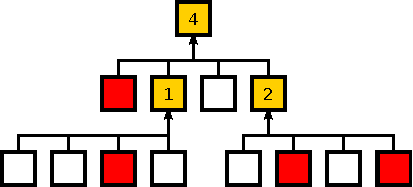
\epsfig{file=figures/CellLocking.pdf,width=0.5\textwidth}}
    
    \caption{Example of hierarchical cell locking. The cells marked in red
        are ``locked'' while the cells marked in yellow have a ``hold'' count
        larger than zero.
        The hold count is shown inside each cell and corresponds to the number
        of locked cells hierarchicaly below it.
        All cells except for those locked or with a ``hold'' count larger than
        zero can still be locked without causing concurrent data access.
        }
    \label{fig:CellLocking}
\end{figure}


%%%%%%%%%%%%%%%%%%%%%%%%%%%%%%%%%%%%%%%%%%%%%%%%%%%%%%%%%%%%%%%%%%%%%%%%%%%%%%%%
%  Validation of the algorithms
%%%%%%%%%%%%%%%%%%%%%%%%%%%%%%%%%%%%%%%%%%%%%%%%%%%%%%%%%%%%%%%%%%%%%%%%%%%%%%%%
\section{Validation}

\subsection{Implementation details}

\begin{itemize}

    \item Implemented in C, compiled with {\tt gcc}.

    \item Threading implemented with {\tt pthread}.

    \item One task queue per thread.
    
    \item As of yet, no use of SIMD capabilities to evaluate several
        interactions at a time.
    
    \item Details of the pair interactions.
    
    \item Details of the hardware.
        
\end{itemize}


\subsection{Simulation setup}

\begin{itemize}

    \item Details of the simulation used, e.g. size, number of particles,
        etc...
        
    \item So far only considering density and force computation,
        particles not moving.
        
\end{itemize}


\subsection{Results}

\begin{itemize}

    \item Scaling for both simulations on different parallel hardware.
    
    \item Compare, if possible, with {\sc gadget}.
        
\end{itemize}


%%%%%%%%%%%%%%%%%%%%%%%%%%%%%%%%%%%%%%%%%%%%%%%%%%%%%%%%%%%%%%%%%%%%%%%%%%%%%%%%
%  Conclusions
%%%%%%%%%%%%%%%%%%%%%%%%%%%%%%%%%%%%%%%%%%%%%%%%%%%%%%%%%%%%%%%%%%%%%%%%%%%%%%%%
\section{Conclusions}

\begin{itemize}

    \item Good scaling.
    
    \item Computational model can easily be exported to other architectures,
        including GPUs (reference task-based parallelism on GPUs with Aidan),
        and other multi-core accelerators such as the Intel MIC.
        
\end{itemize}


%%%%%%%%%%%%%%%%%%%%%%%%%%%%%%%%%%%%%%%%%%%%%%%%%%%%%%%%%%%%%%%%%%%%%%%%%%%%%%%%
%  Acknowledgments
%%%%%%%%%%%%%%%%%%%%%%%%%%%%%%%%%%%%%%%%%%%%%%%%%%%%%%%%%%%%%%%%%%%%%%%%%%%%%%%%
\section*{Acknowledgments}

\begin{itemize}

    \item Collaboration with Matthieu Schaller and Tom Theums from the
        Institute of Computational Cosmology (ICC) at Durham University.
        
    \item Lydia Heck from the ICC for providing access to the infrastructure.

\end{itemize}


%%%%%%%%%%%%%%%%%%%%%%%%%%%%%%%%%%%%%%%%%%%%%%%%%%%%%%%%%%%%%%%%%%%%%%%%%%%%%%%%
%  Bibliography
%%%%%%%%%%%%%%%%%%%%%%%%%%%%%%%%%%%%%%%%%%%%%%%%%%%%%%%%%%%%%%%%%%%%%%%%%%%%%%%%
\nopagebreak
\bibliography{sph}



\end{document}
